RC, står for Resistor og Kapasitor (motstand og kondensator).
Og en RC-krets er simpelthen kretser
som består av motstander og kondensatorer.

\begin{circuitikz} \draw
(0,0) to[vsourcesin] (0,2)
      to[R] (4,2)
      to[C] (4,0)
      -- (0,0)
      ;
\end{circuitikz}



\paragraph{Spenning og impedans} \mbox{} \\
Husk at strømmen i en kondensator ligger 90 grader forran spenningen.
Det vil si at spenningen over en kondensator ligger forskøvet
90 grader i forhold til spenningen i en motstand.
Vektorsummen gir den totale spenningen.
\\
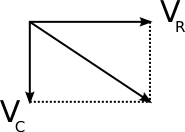
\includegraphics[width=0.25\textwidth]{./img/spenningRC}
\\
I en krets med en motstand og en kondensator i serie gir dette oss
$$V_T = \sqrt{V_R^2 + V_C^2}$$
Og tilsvarende for impedansen.
$$Z_T = \sqrt{R^2 + X_C^2}$$


\paragraph{Eksempel} \mbox{} \\
Finn den totale impedansen Z
for en seriekoblet motstand, kondensator og vekselstrømkilde.\\
$R = \SI{25}{k\ohm}$ \qquad
$C = \SI{6}{n\farad}$ \qquad
$f = \SI{2}{k\hertz}$
\\
$$X_C = \frac{1}{2\pi \cdot f \cdot C}
= \frac{1}{2\pi \cdot 2\cdot 10^3\cdot 6\cdot 10^{-9}} = \SI{13,3}{k\ohm}$$
\\
$$Z = \sqrt{R^2 + X_C^2}
= \sqrt{(25 \cdot 10^3)^2 + (13,3 \cdot 10^3)^2} = \SI{28,3}{k\ohm}$$



\paragraph{Tidskonstant} \mbox{} \\
Når en ladet kondensator står i en lukket krets med motstand,
vil kondensatoren lade seg ut.
\\\\
\begin{circuitikz} \draw
(0,0) to[C, label=$C$] (0,2)
      -- (4,2)
      to[R, label=$R$] (4,0)
      -- (0,0)
      ;
\end{circuitikz}
\\\\
Spenningen U  er gitt ved $U = R \cdot I$.
\\
Spenningen til kondensatoren kaller vi V.
\\
Etter kirchhoffs lov om spenninger er
summen av alle spenninger i en krets lik null.
\\
$$R \cdot I + V = 0$$
\\\\
Strøm I er gitt ved
$$I = C \cdot \frac{dV}{dt}$$
\\\\
Satt inn for I gir det
$$R \cdot C \cdot \frac{dV}{dt} + V = 0$$
\\\\
Løser man dette for spenningen over kondensatoren får man
$$V_C(t) = V_0 \cdot e^{\frac{-t}{RC}} = V_0 \cdot e^{\frac{-t}{\tau}}$$
Hvor $\tau = RC$ er \emph{tidskonstanten}.
\\\\
Etter en tid $\tau$ har størrelsen blitt redusert
til ca 37\% av startverdien.
Etter $5 \tau$ er størrelsen redusert til 1\%
og kondensatoren anses som utladet.
\\
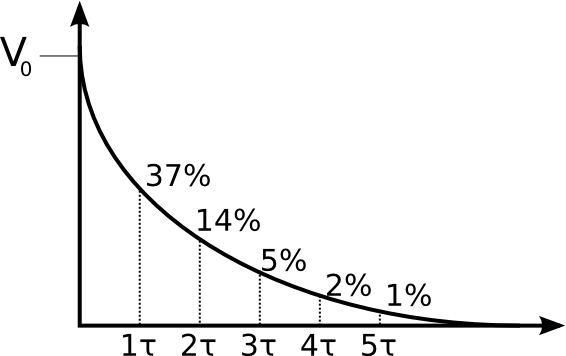
\includegraphics[width=0.5\textwidth]{./img/tidskonstant}

